\documentclass[14pt, a0paper, landscape]{tikzposter}
\usepackage[sfmath]{kpfonts}
\usepackage[default]{gillius}
\usepackage[backend=biber, style=authoryear, uniquelist=minyear, uniquename=false]{biblatex}
\usepackage{multirow}
\usepackage{capt-of}
\usepackage{adjustbox}
\graphicspath{{../figures/}}
\usetheme{Board}

\addbibresource{papers.bib}
\setlength{\bibhang}{0pt}

\title{Phylogenetic estimation of contact network parameters with kernel-ABC}
\author{Rosemary M. McCloskey$^1$ and Art F. Y. Poon $^{1,2}$}
\date{March 11, 2015}
\institute{$^1$ BC Centre for Excellence in HIV/AIDS 
           $^2$ Department of Medicine, University of British Columbia}
\begin{document}

\maketitle

\begin{columns}
  \column{0.25}
  \block{Contact networks shape viral transmission trees}{
    \centerline{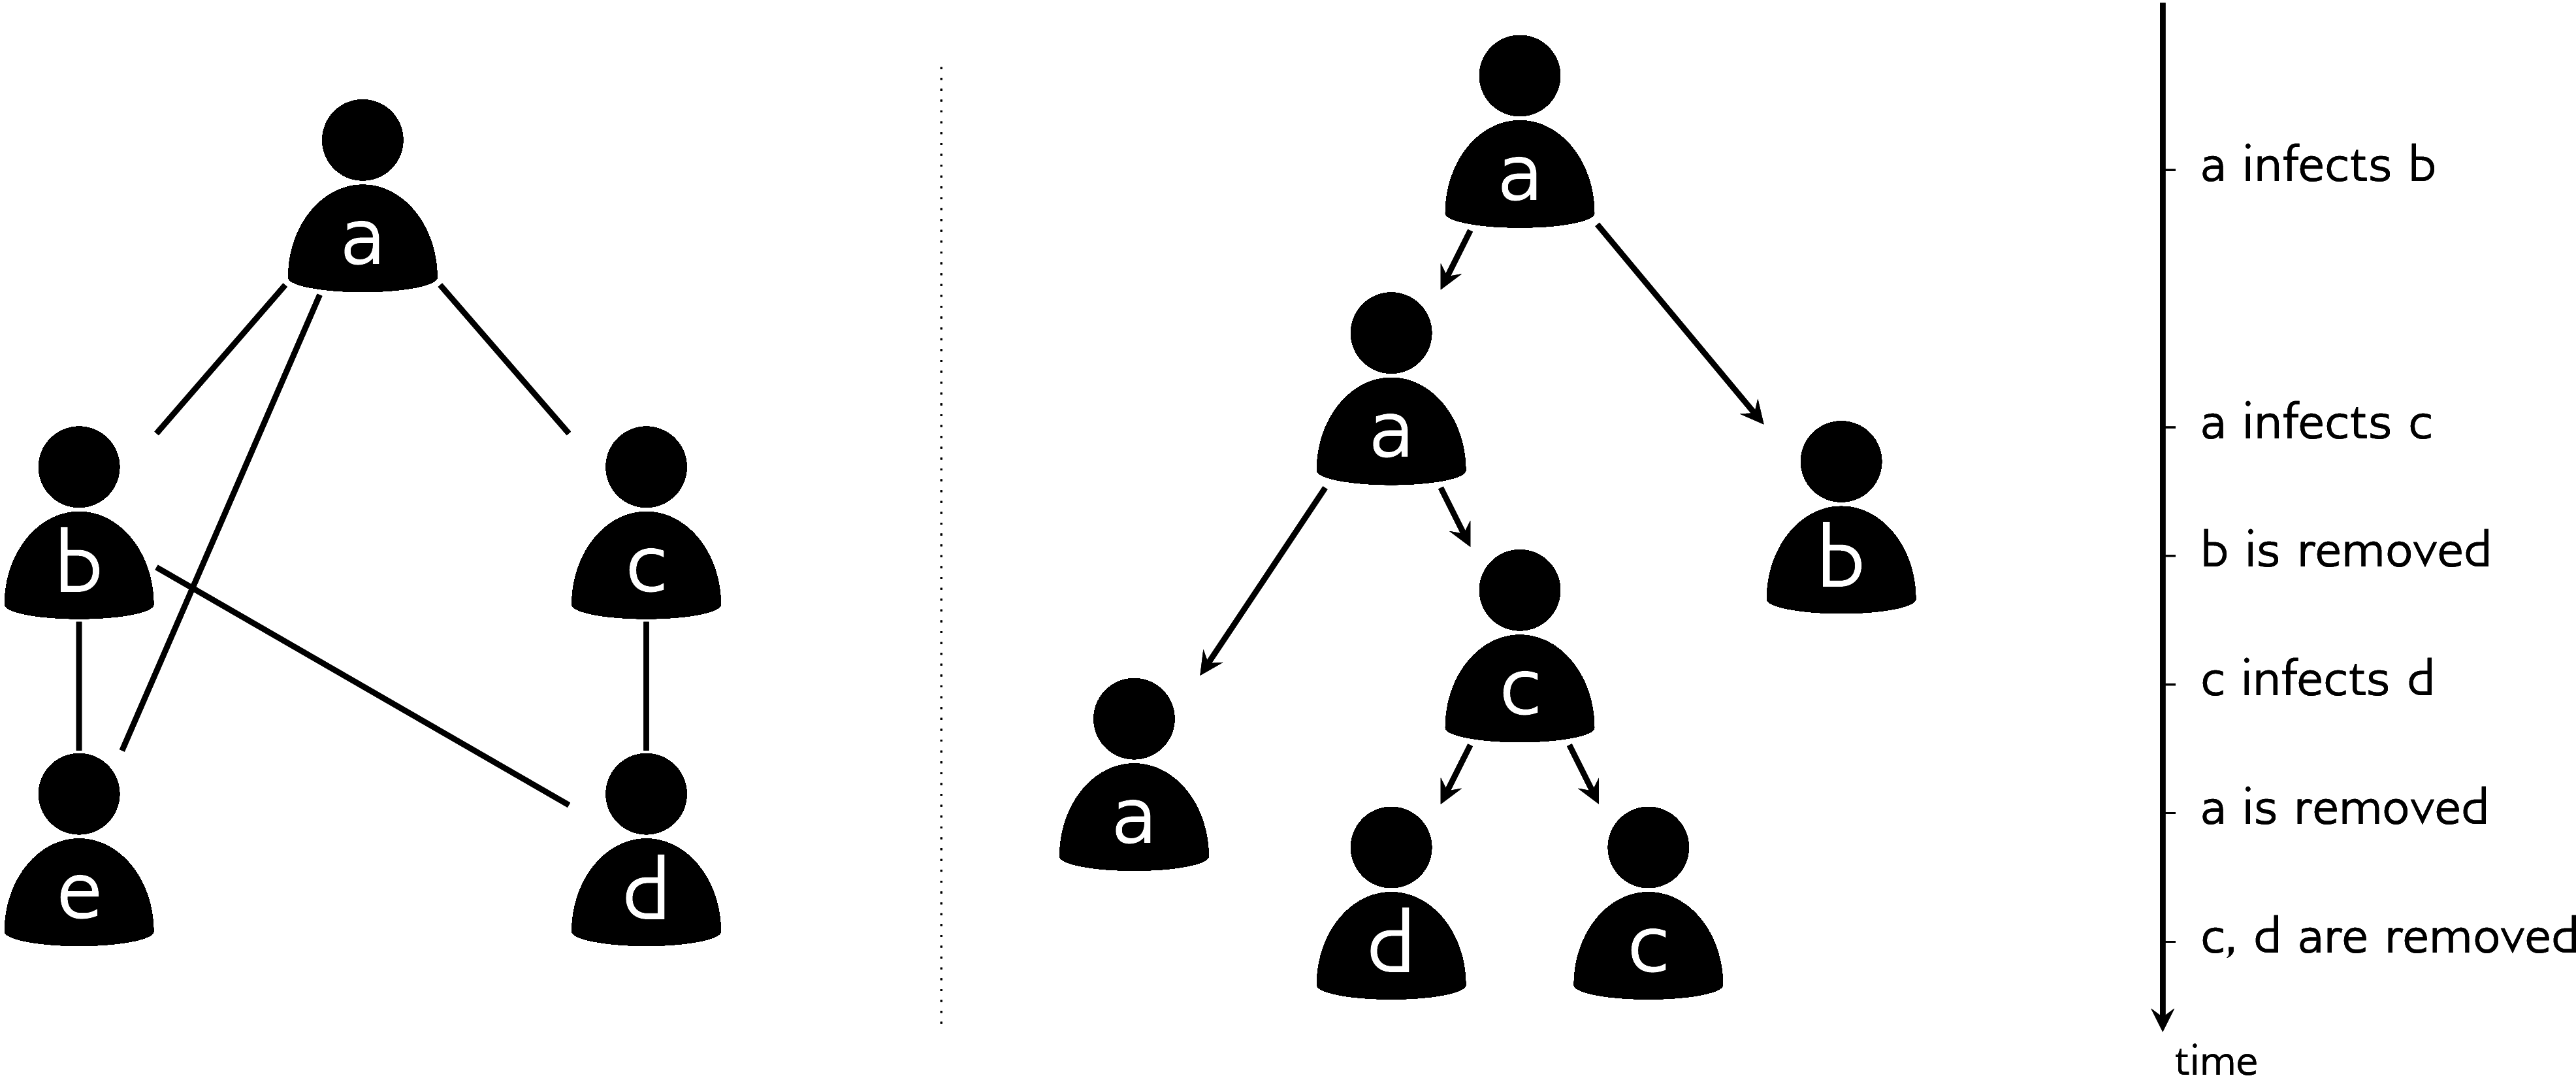
\includegraphics[width=0.2\textwidth]{contactnet}}
  }
  \block{What can we tell about contact networks from viral sequence data?}{
  }

  \block{Barab\'asi-Albert preferential attachment networks}{

    \begin{itemize}
      \item Nodes are added one-at-a-time until there are $N$ total.
      \item Each time a node is added, $m$ new edges are connected to it.
      \item Each new edge is attached to an existing node of degree $d$ with
        probability proportional to $d^\alpha$.
    \end{itemize}

    \vspace{1cm}
    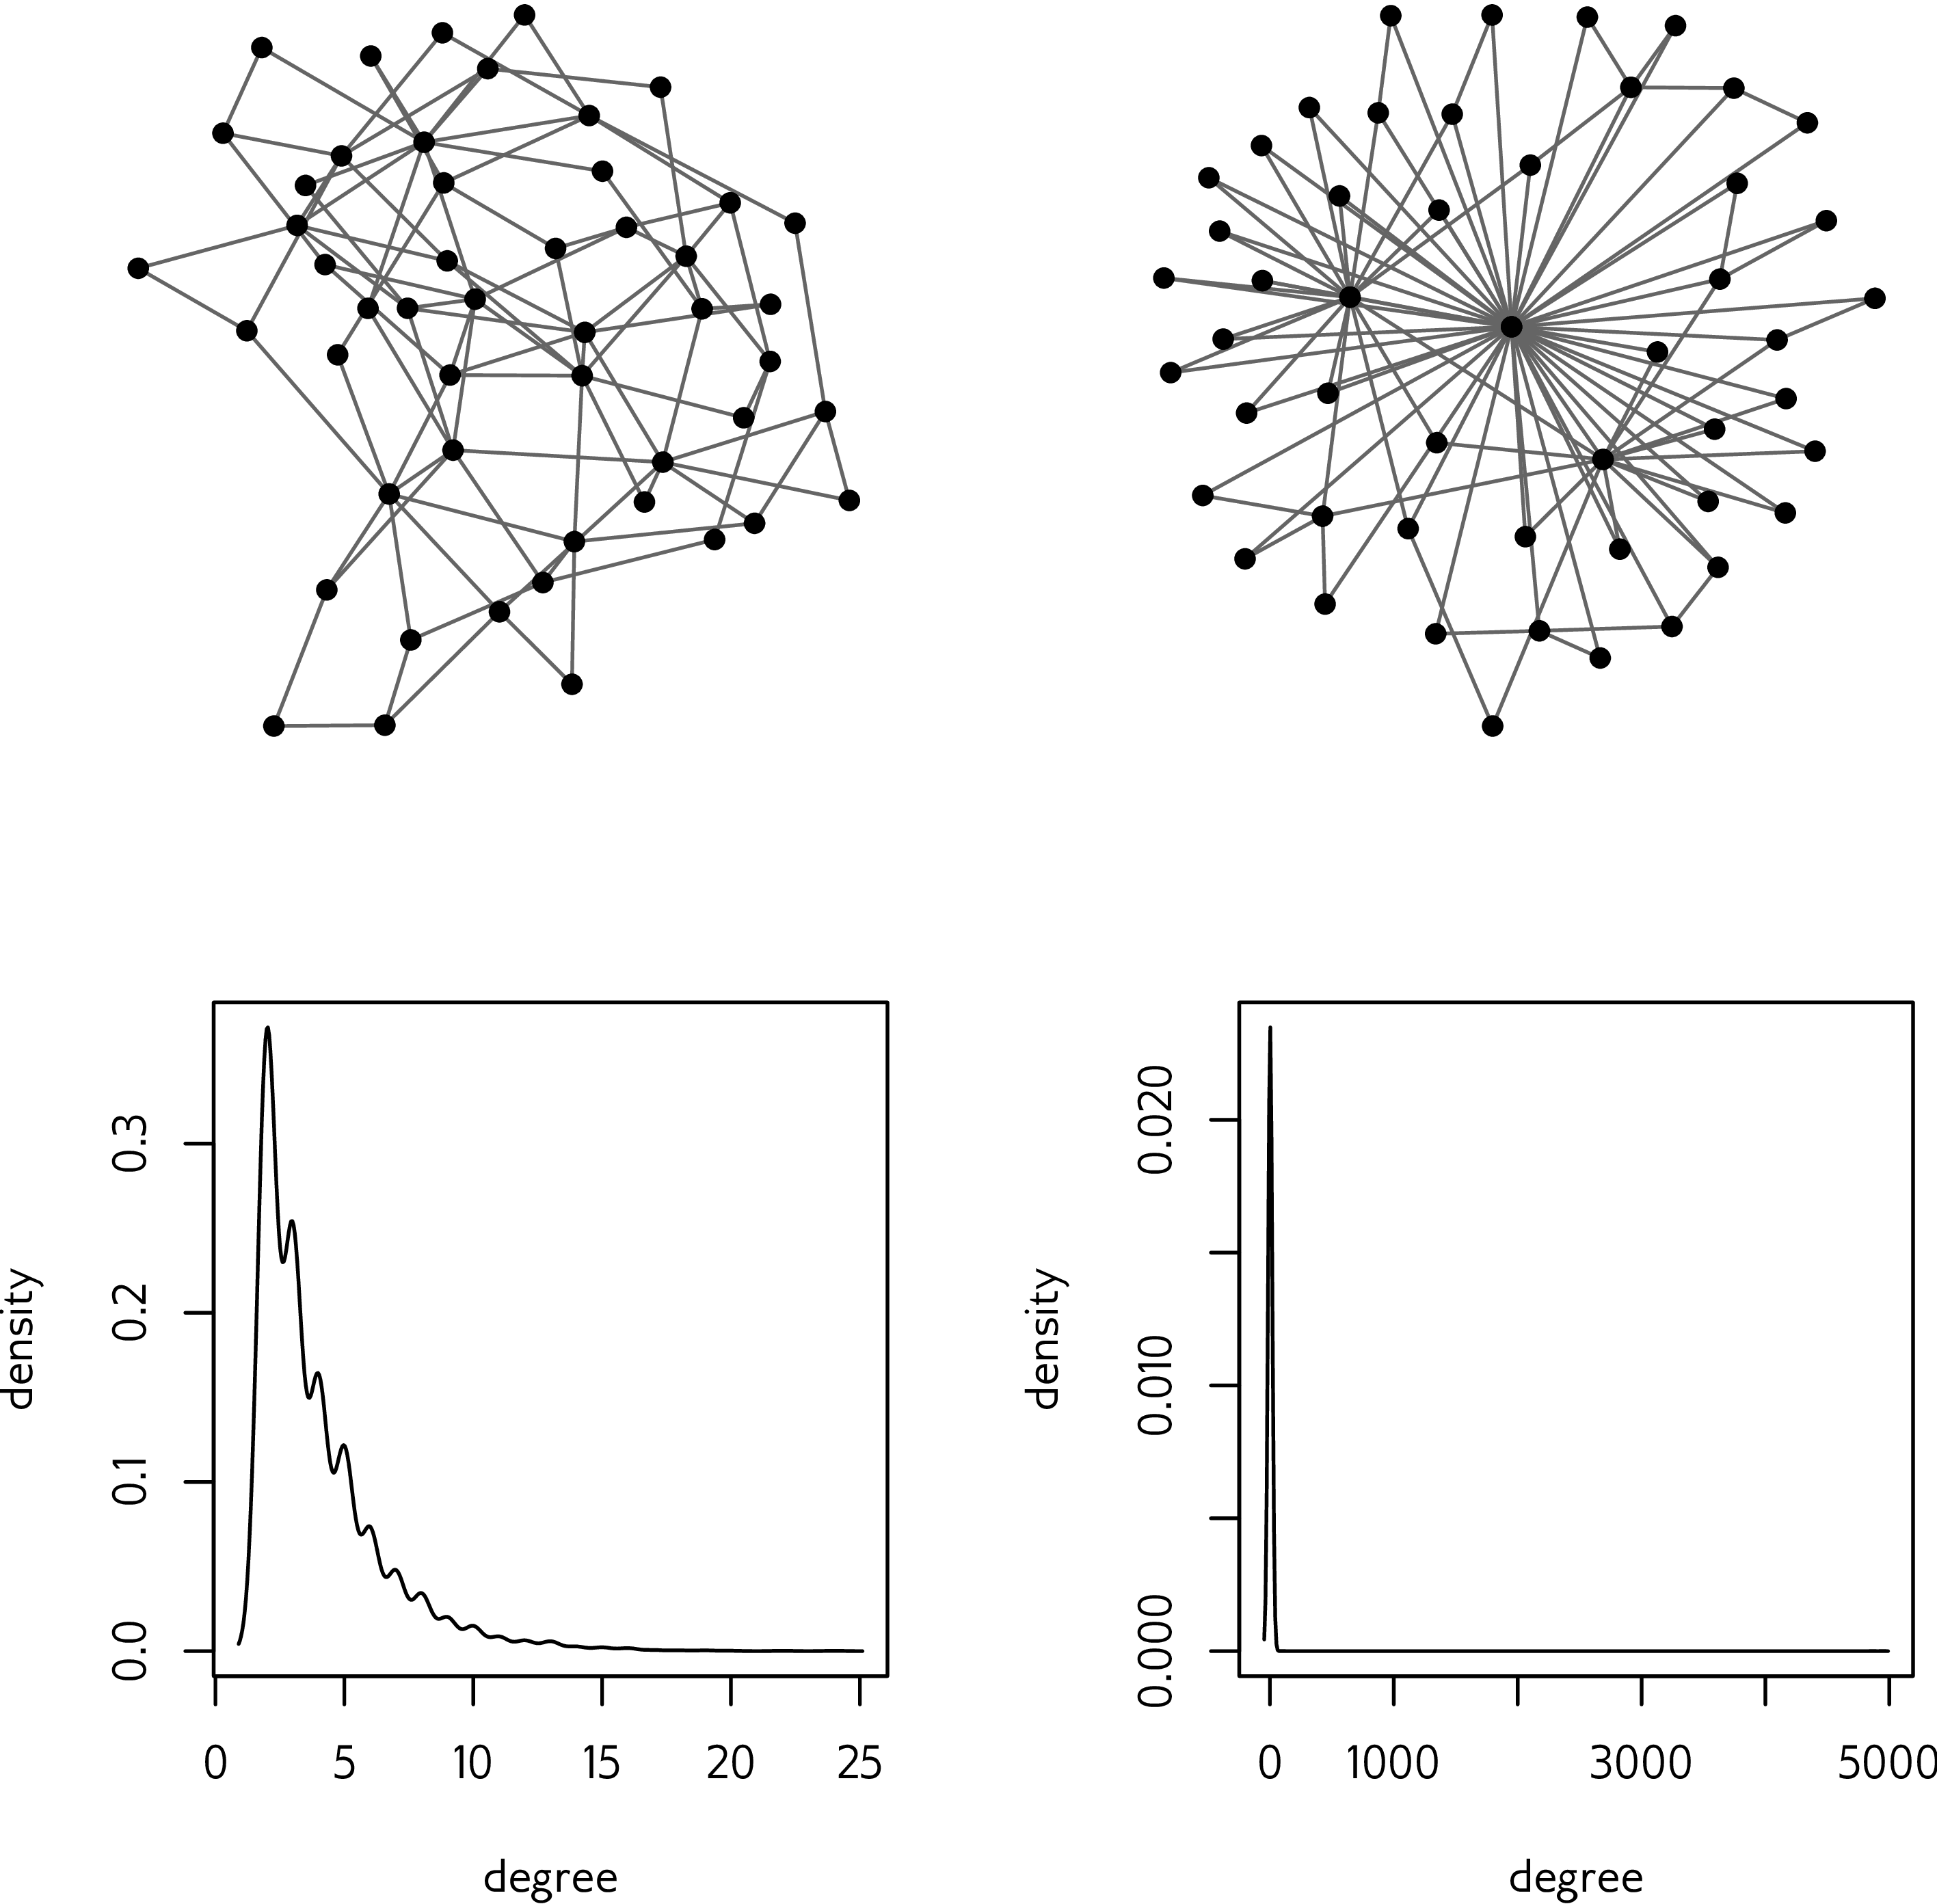
\includegraphics[width=0.2\textwidth, trim=0 22in 0 0, clip]{alpha-bounds}
    \begin{center}
      \begin{tabular}{cl}
        parameter & meaning \\
        \hline
        $\alpha$ & preferential attachment power: nodes of degree $d$ attract new edges with probability $\propto d^\alpha$ \\
        $m$ & number of new edges added for each new vertex \\
        $I$ & number of infected nodes when epidemic simulation is stopped \\
        $N$ & total number nodes in the network \\
        \hline
      \end{tabular}
    \end{center}
  }

  \block{Approximate Bayesian computation}{
  }

  \column{0.25}
  \block{Phylogenetic kernel lets us compare tree shapes}{
    \nocite{poon2013mapping}
  }

  \block{ABC with sequential Monte Carlo}{
    \centerline{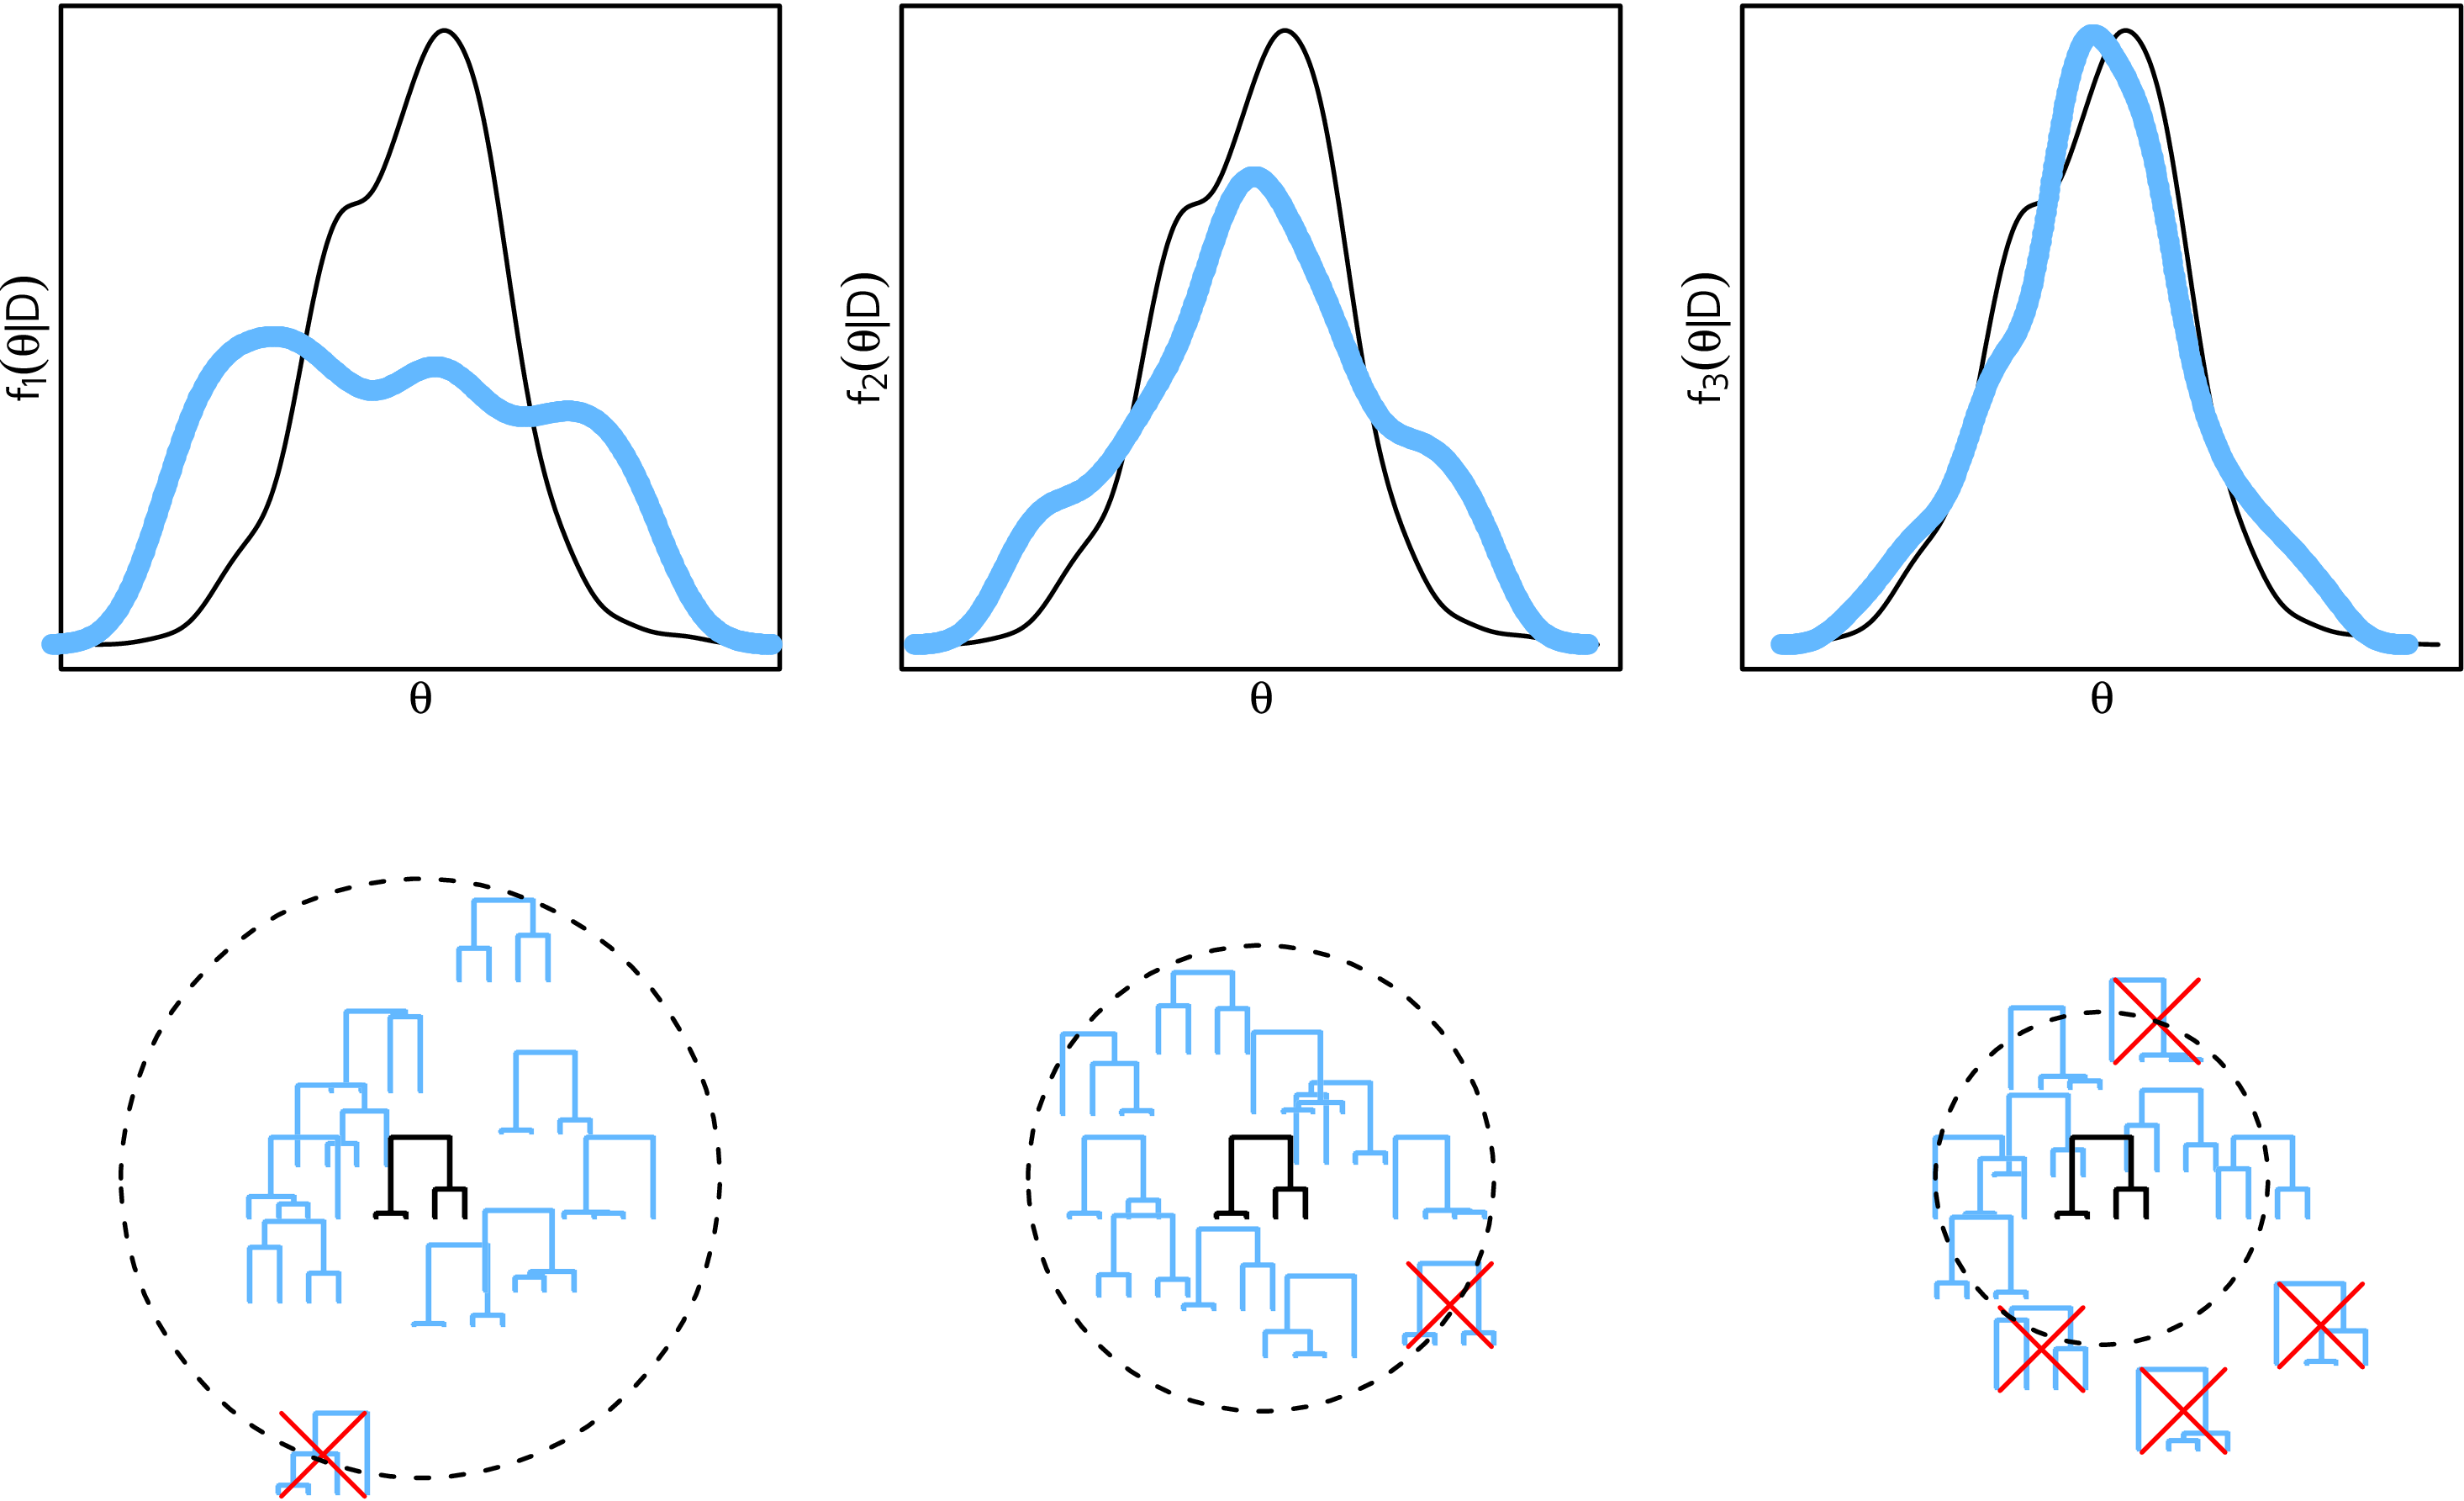
\includegraphics[width=0.2\textwidth]{abc-smc}}
    \nocite{del2012adaptive}
  }

  \block{Varying $\alpha$ and $I$ affects tree shape, but not $m$ and $N$}{
    \centerline{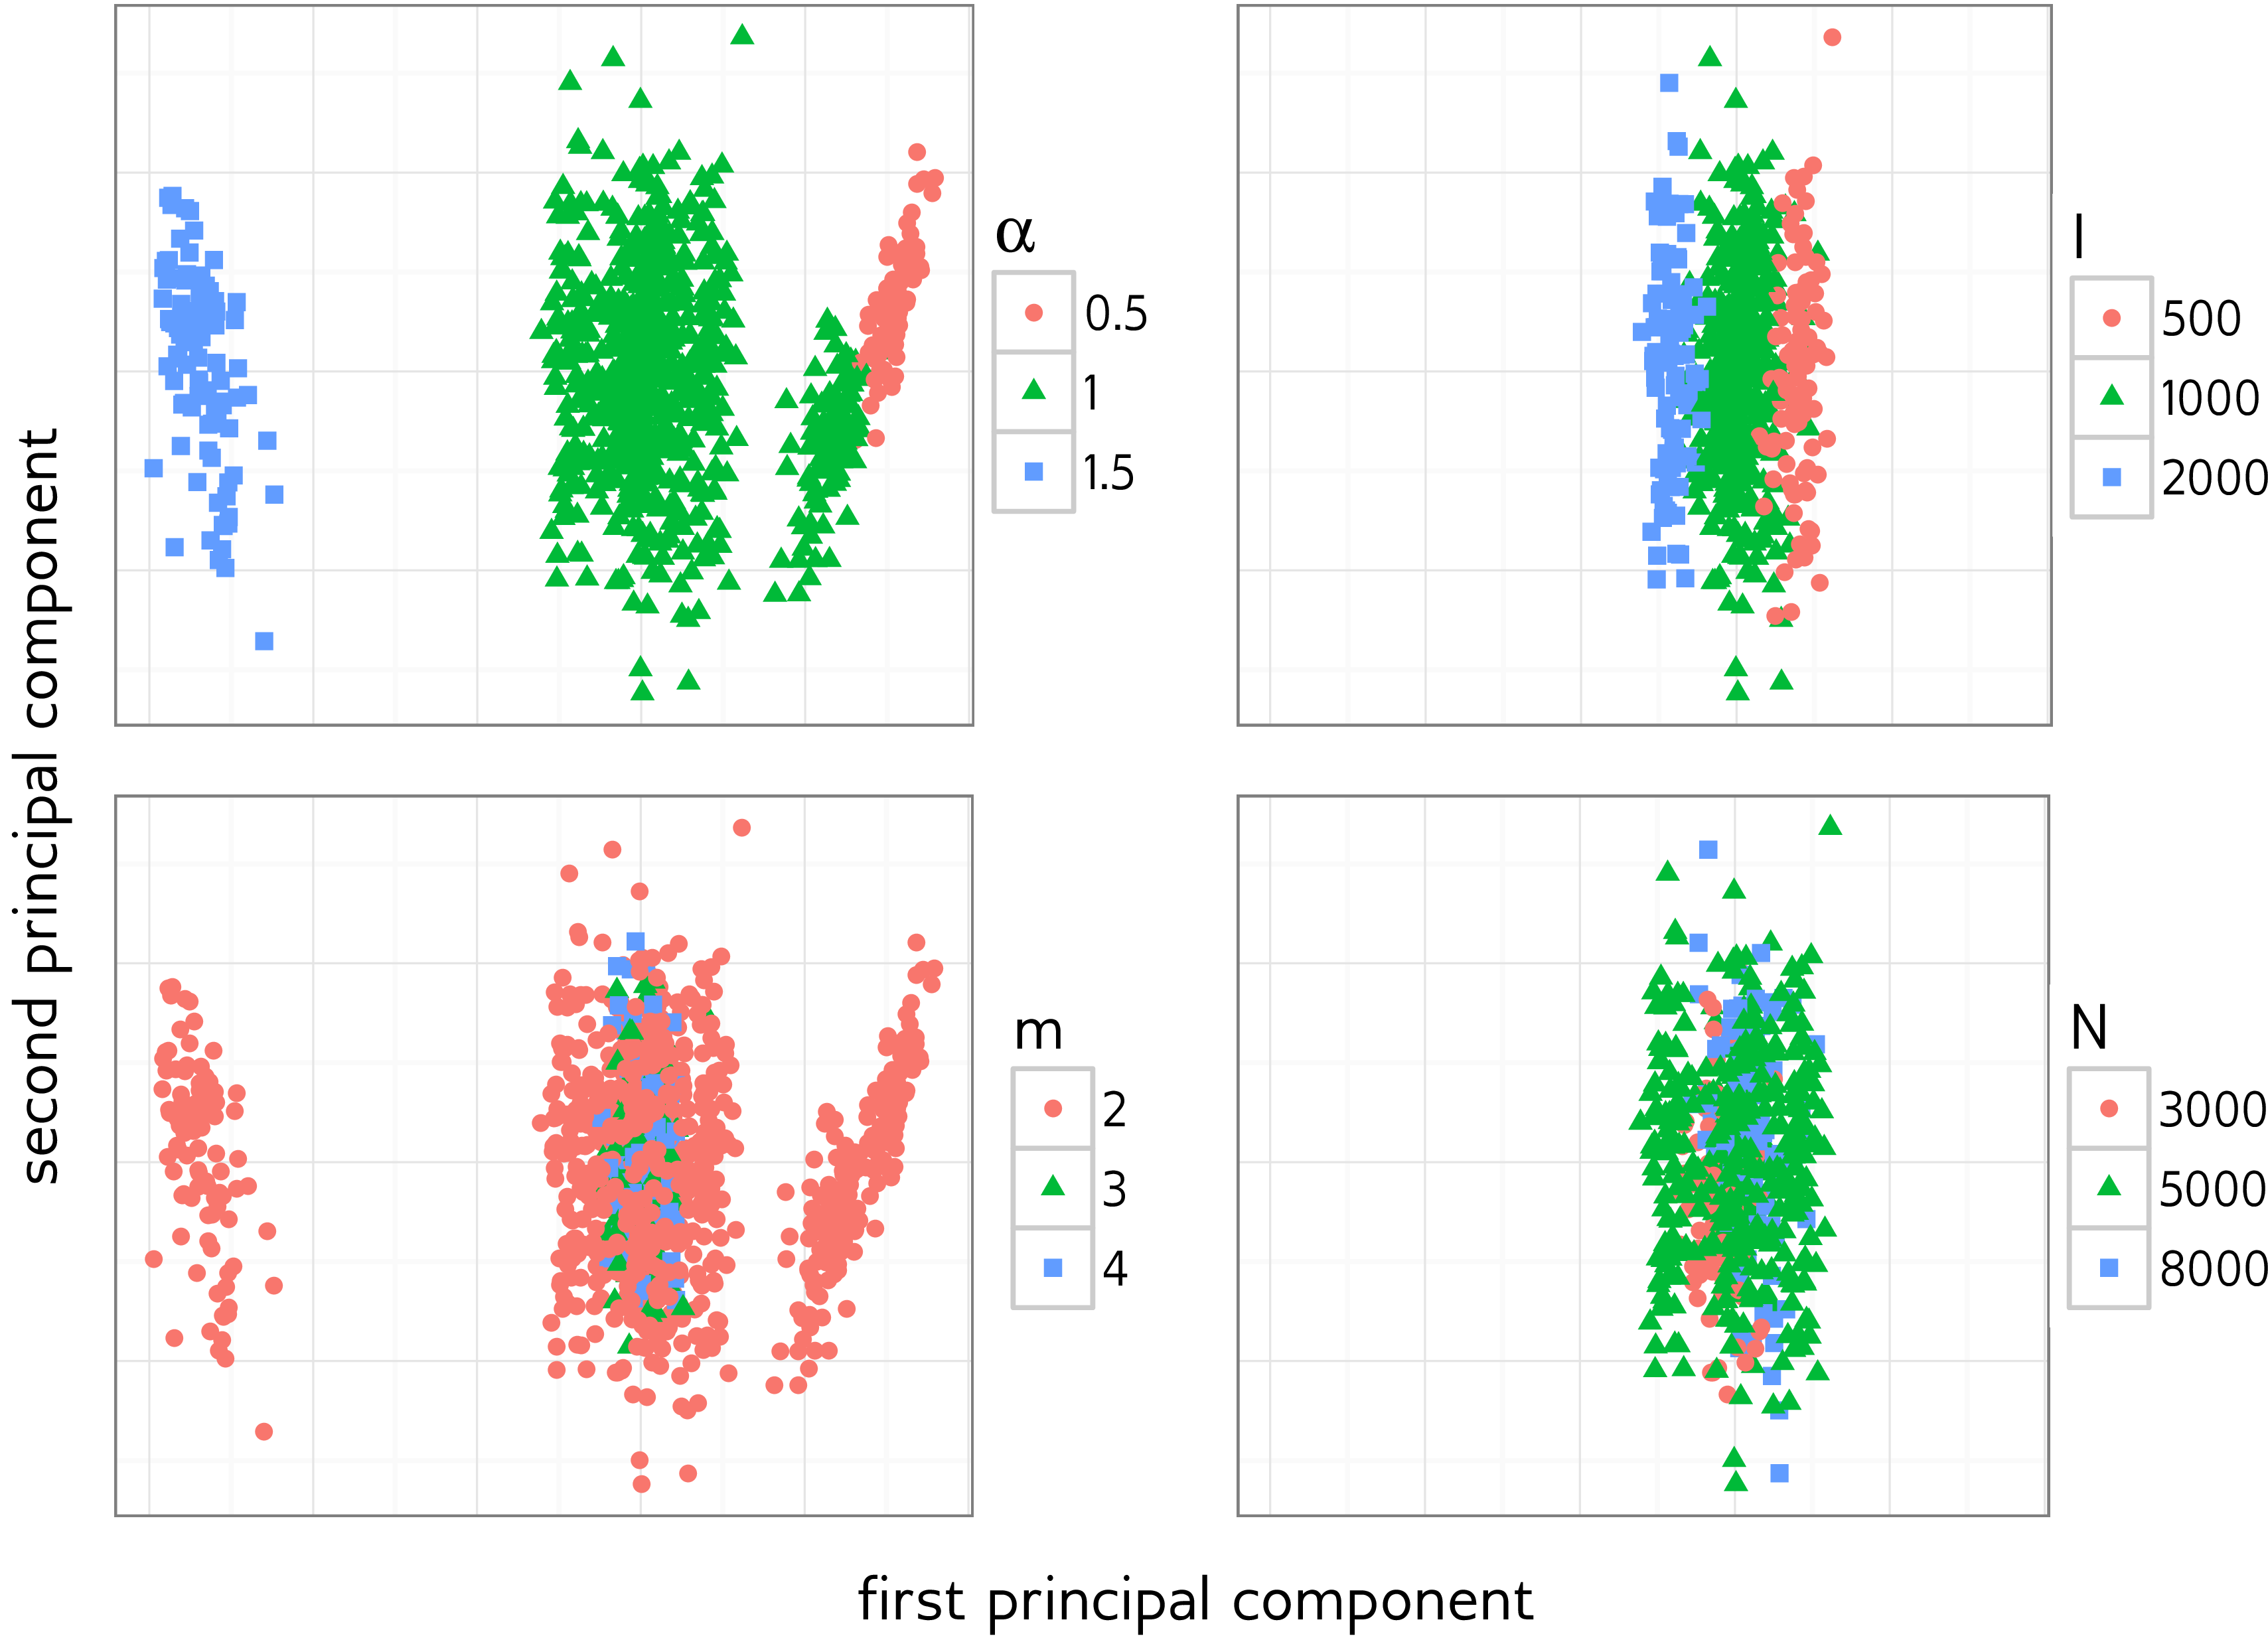
\includegraphics[width=0.2\textwidth]{kernel-kpca}}
  }

  \column{0.25}
  \block{Simulations}{
    \begin{minipage}[t]{0.5\linewidth}
      \begin{tabular}{ccc}
        parameter & values & prior \\
        \hline
        $\alpha$ & 0.0, 0.5, 1.0, 1.5 & Uniform(0, 2) \\
        $m$ & 2, 3, 4 & Uniform(1, 6) \\
        $I$ & 1000, 2000 & Uniform(500, 5000) \\
        $N$ & 5000 & Uniform(500, 15000) \\
        \hline
      \end{tabular}
    \end{minipage}
    \hspace{0.05\linewidth}
    \begin{adjustbox}{valign=t}
      \begin{minipage}[t]{0.45\linewidth}
        Three networks/trees were simulated under each parameter combination.
        Kernel-ABC was used to re-estimate the parameters.
      \end{minipage}
    \end{adjustbox}
  }
  \block{Accurate estimates for $\alpha$, $I$, but not $m$, $N$}{
    \centerline{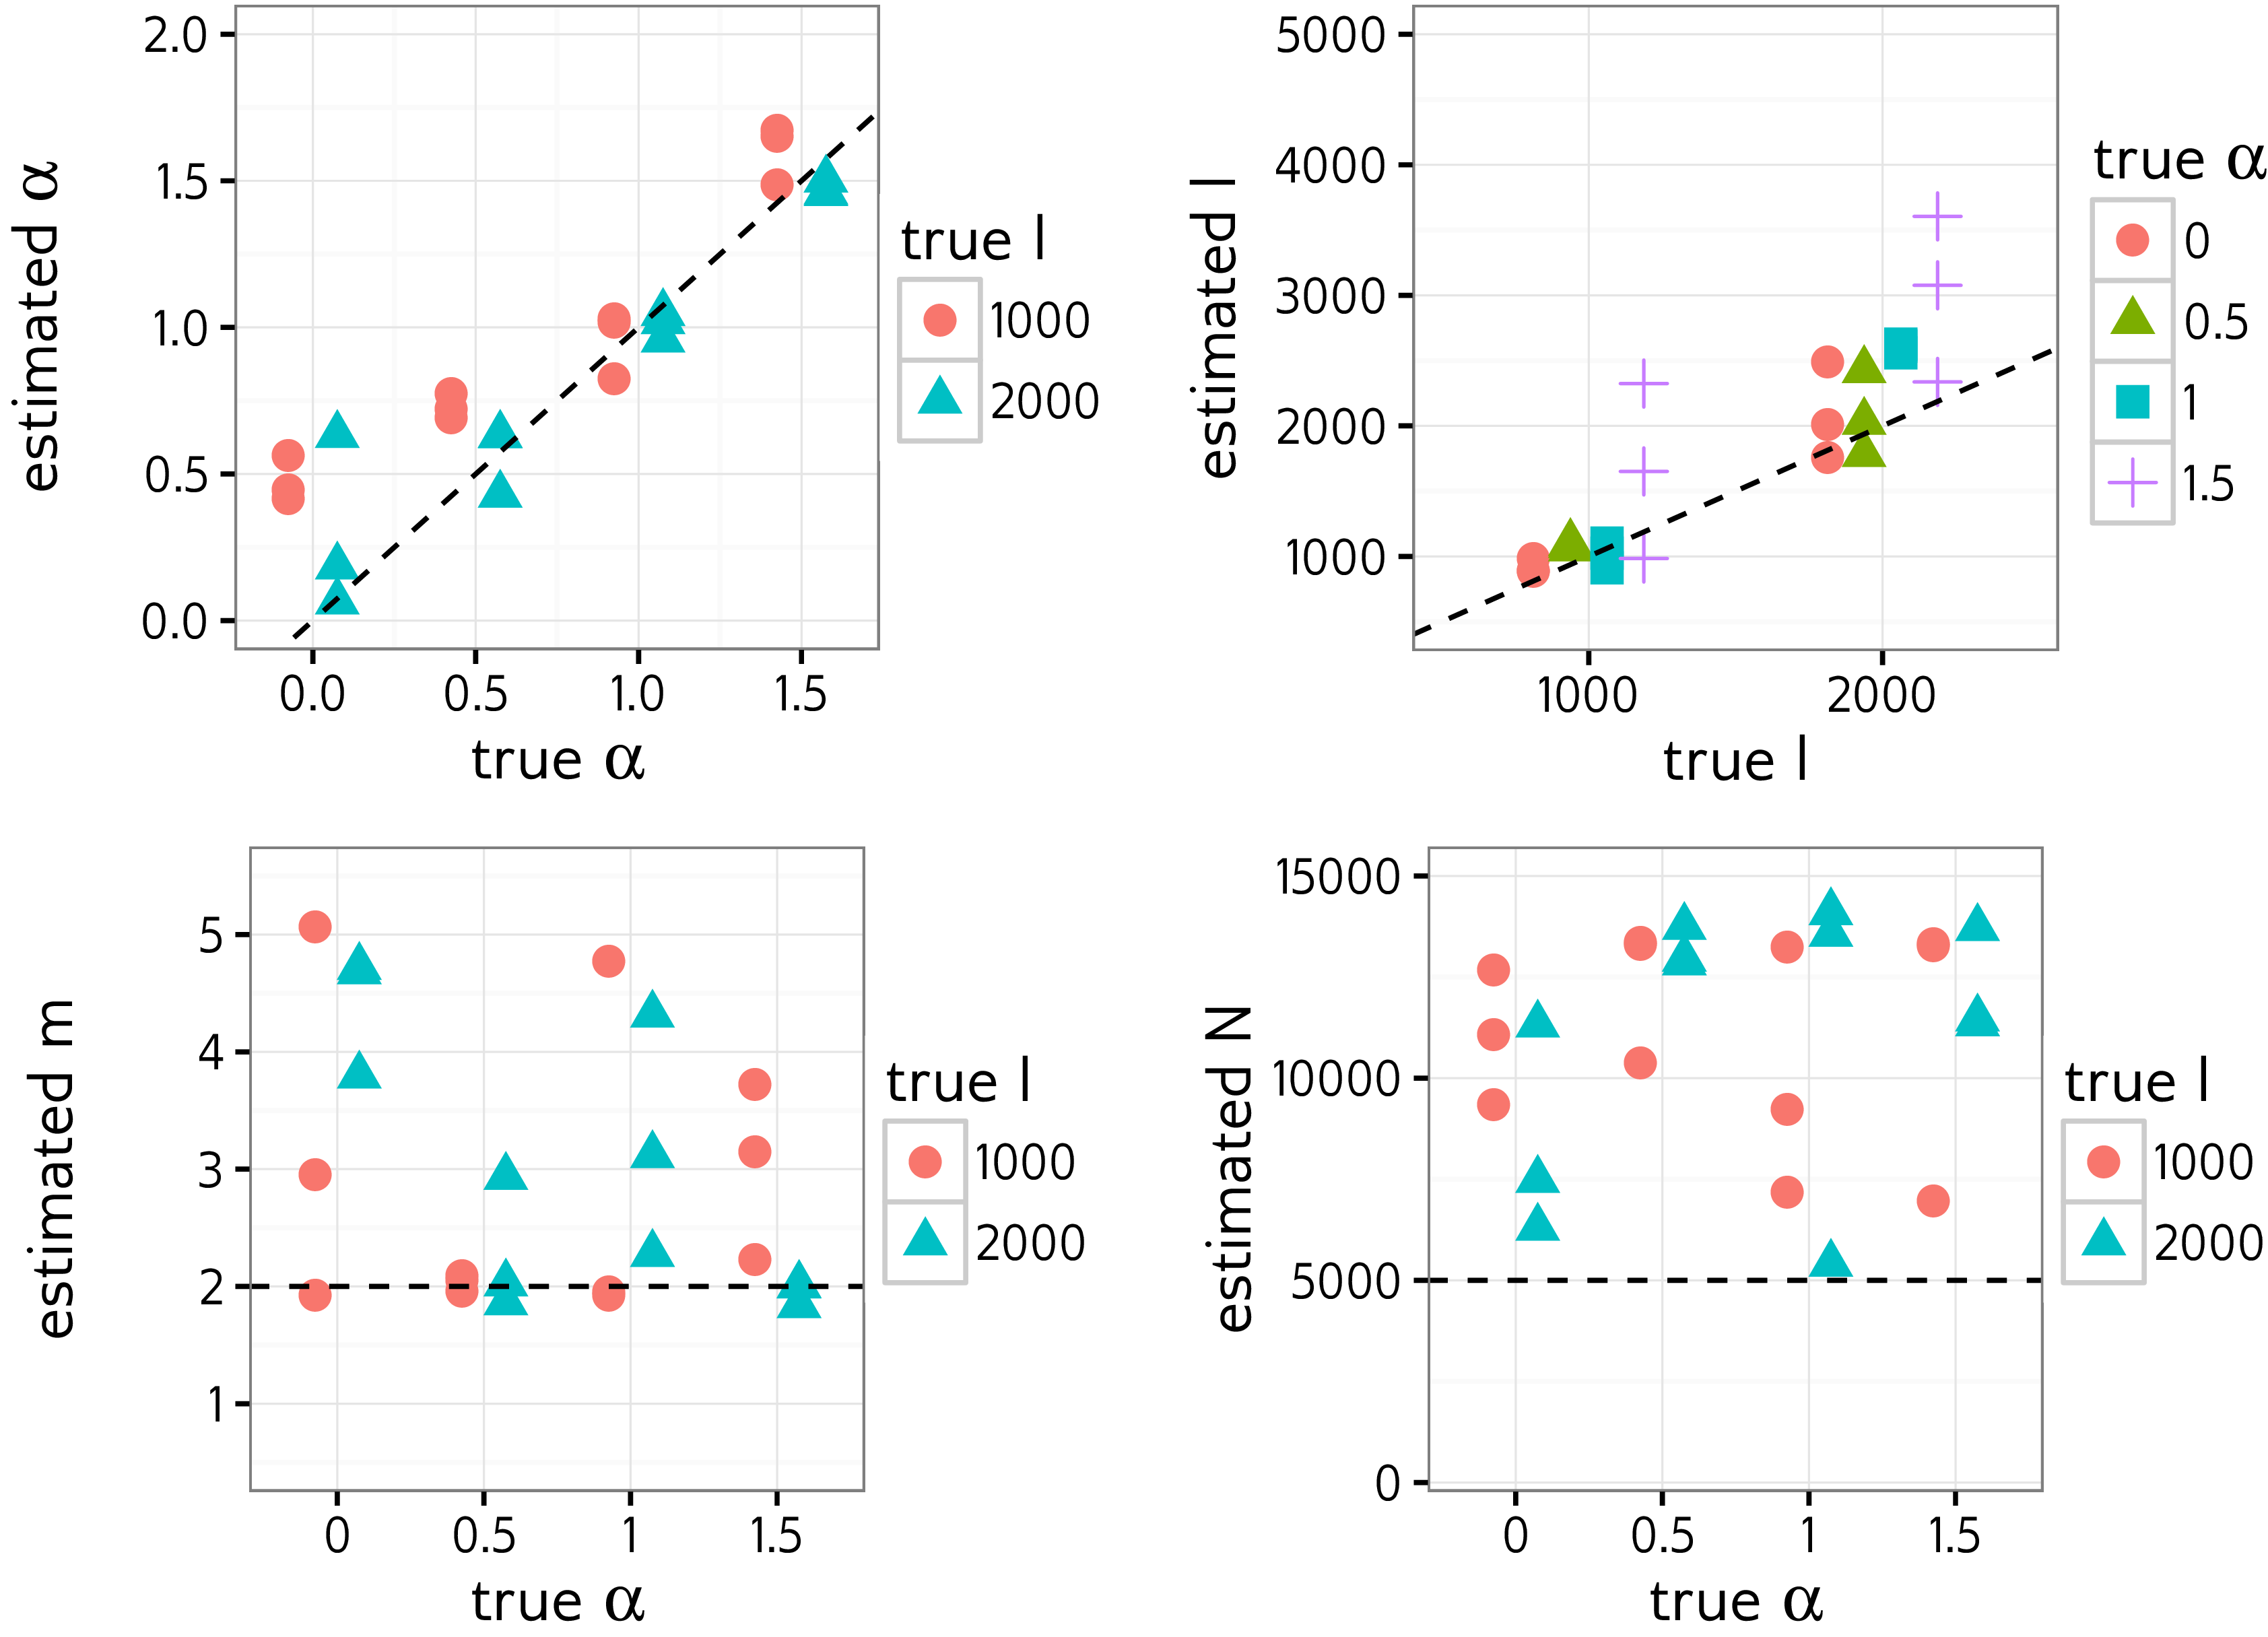
\includegraphics[width=0.2\textwidth]{abc-point-estimate}}
  }
  \block{Narrow dispersion of $\alpha$, $I$ compared to $m$, $N$}{
    \centerline{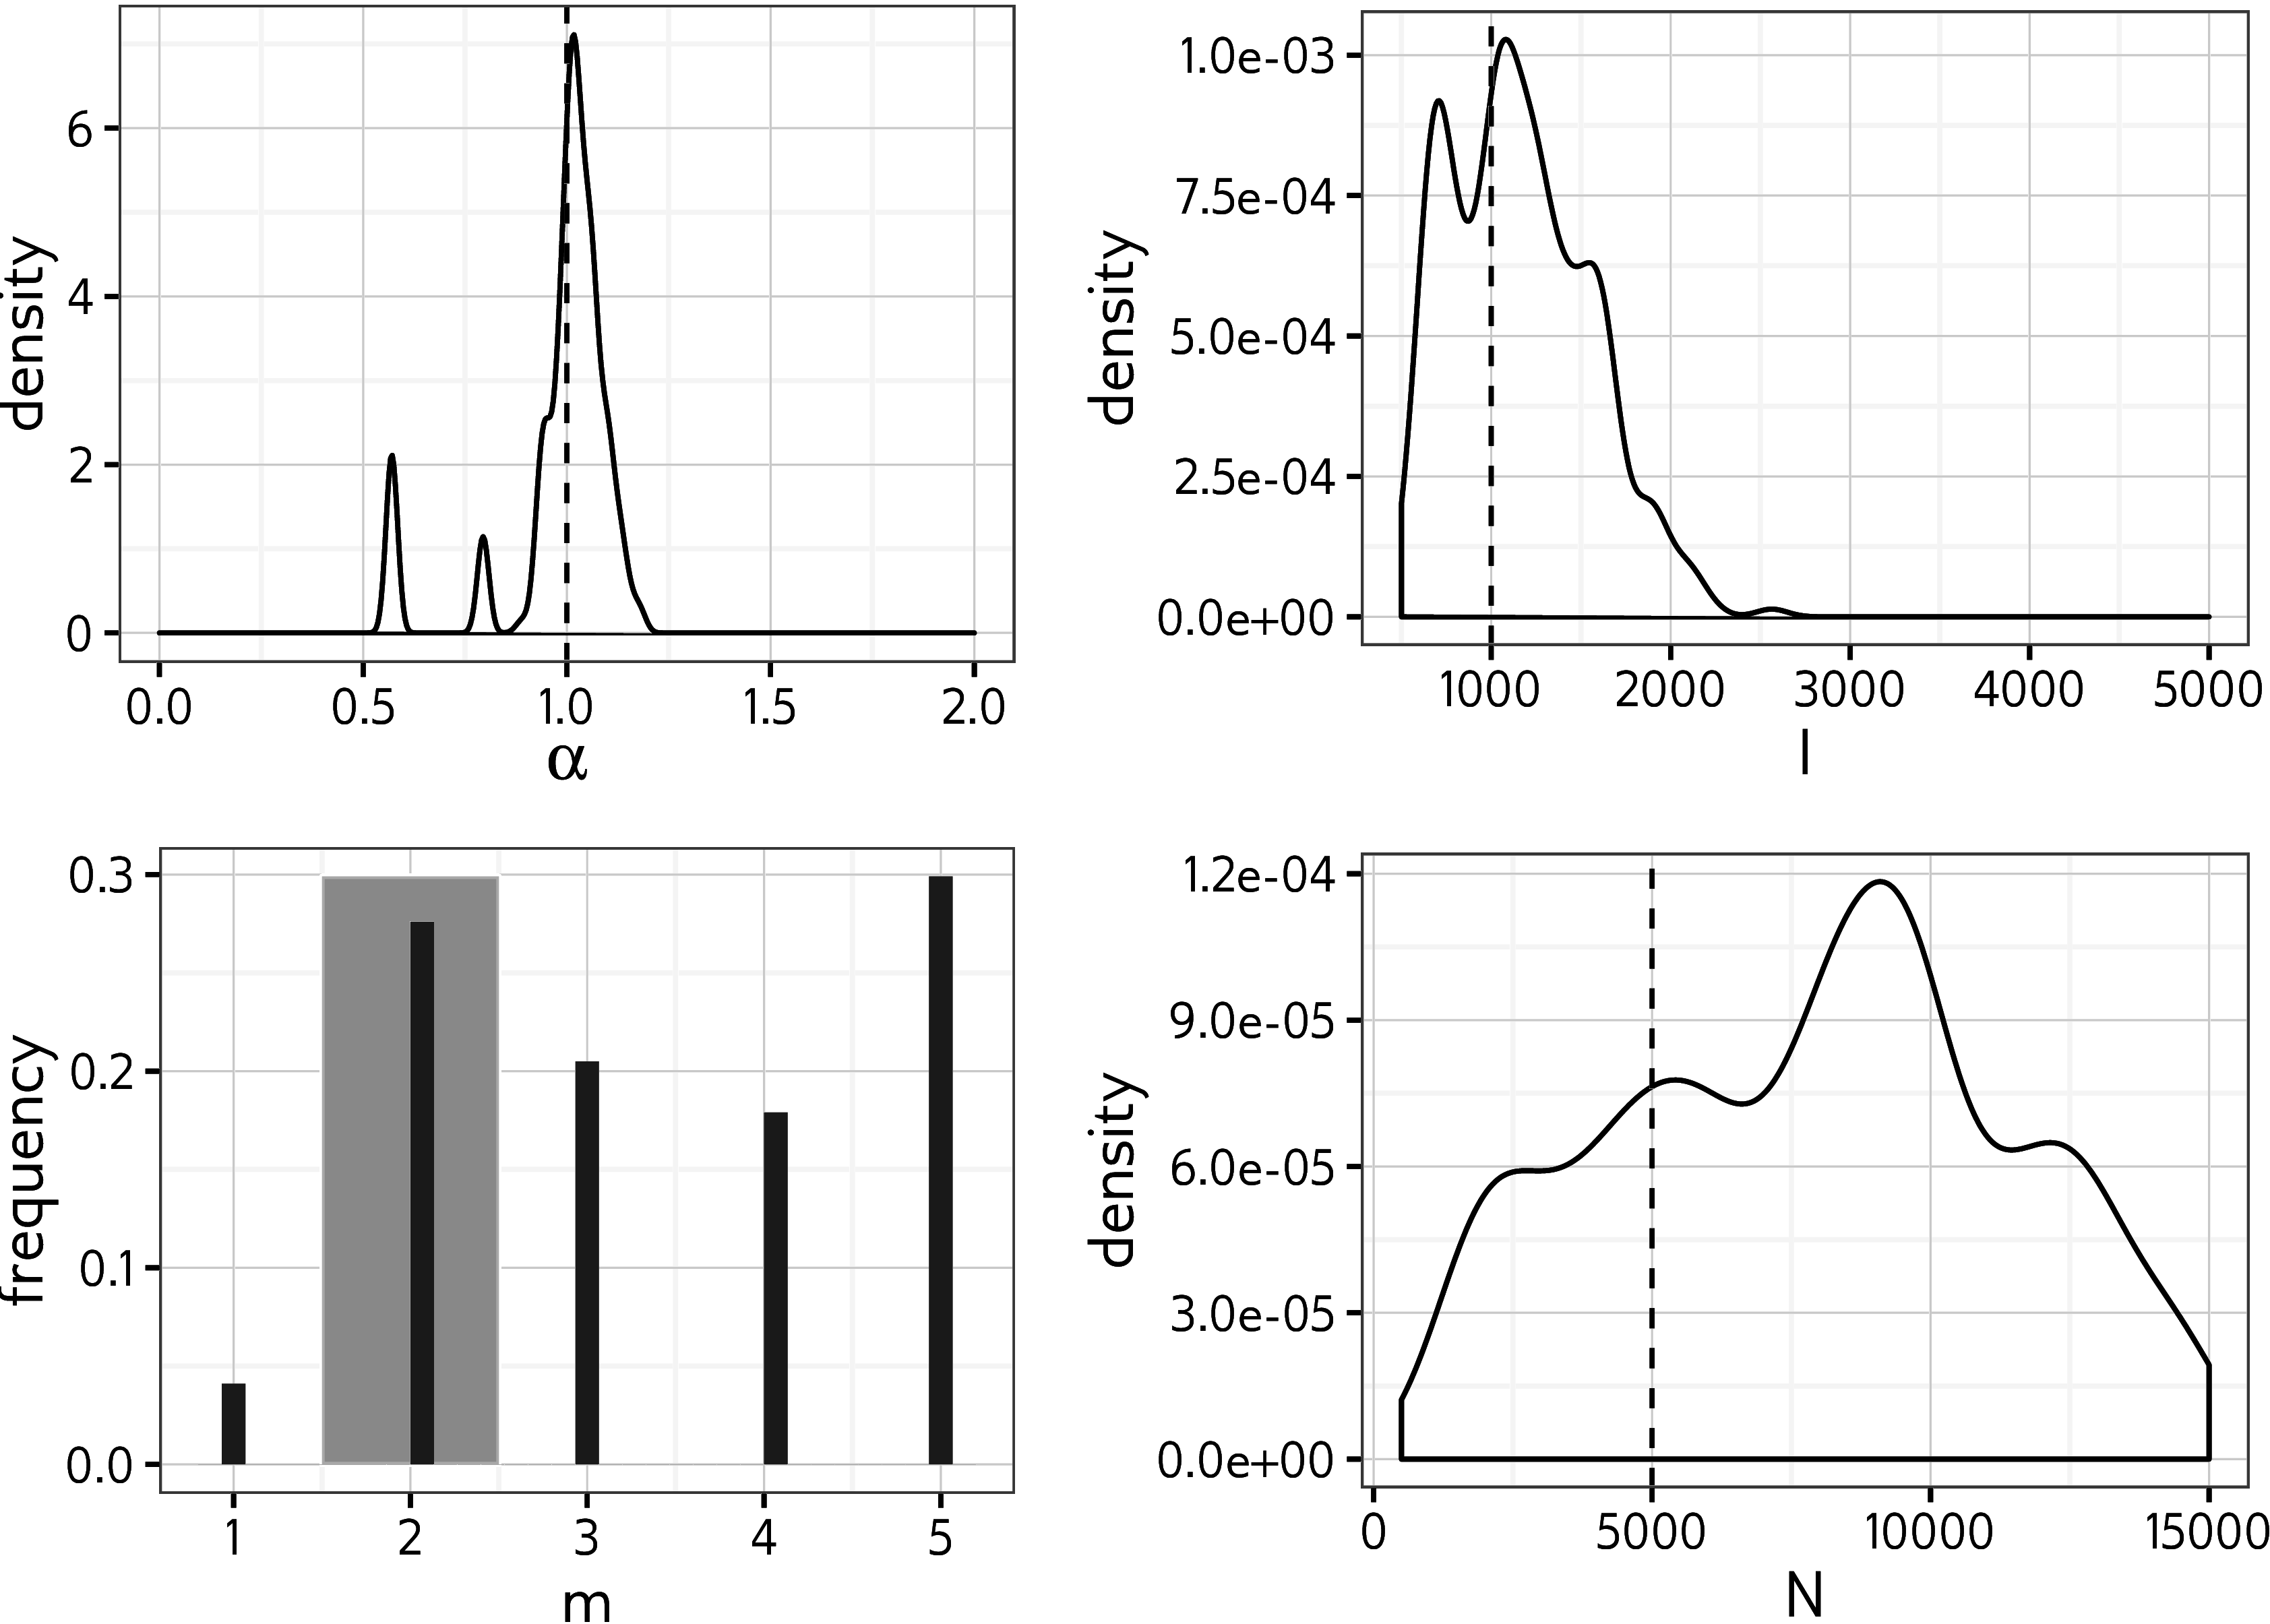
\includegraphics[width=0.2\textwidth]{abc-posterior-example}}
  }

  \column{0.25}

  \block{Real data: phylogenetic and geographic clusters}{
    \centering
    \begin{tabular}{ccccc}
      Reference & Risk group & Sequences ($n$) & Location & HIV gene \\
      \hline
      \textcite{niculescu2015recent} & IDU & 136 & Romania & \textit{pol} \\
      \textcite{li2015hiv} & MSM & 280$^1$ & Shanghai, China & \textit{pol} \\
      \textcite{shiino2014phylodynamic} & mixed & 211$^2$ & Japan & \textit{pol} \\
      \textcite{cuevas2009hiv} & mixed & 287 & Basque Country, Spain & \textit{pol} \\
      \textcite{novitsky2013phylogenetic} & \multirow{2}{*}{mixed} & 
      \multirow{2}{*}{218$^3$} &
      \multirow{2}{*}{Mochudi, Botswana} & 
      \multirow{2}{*}{\textit{env}} \\
      \textcite{novitsky2014impact} \\
      N/A & IDU & 399$^4$ & BC, Canada & \textit{pol} \\
      \hline
    \end{tabular}
    \captionof{table}{
      Characteristics of HIV datasets analysed with kernel-ABC. Abbreviations:
      MSM, men who have sex with men; IDU, injection drug users. $^1$subsampled
      from 1261 $^2$subsampled from 3531 $^3$subsampled from 1299 $^4$subsampled 
      from 7923.}
  }

  \block{Transmission trees were estimated from viral sequence data}{
    \centerline{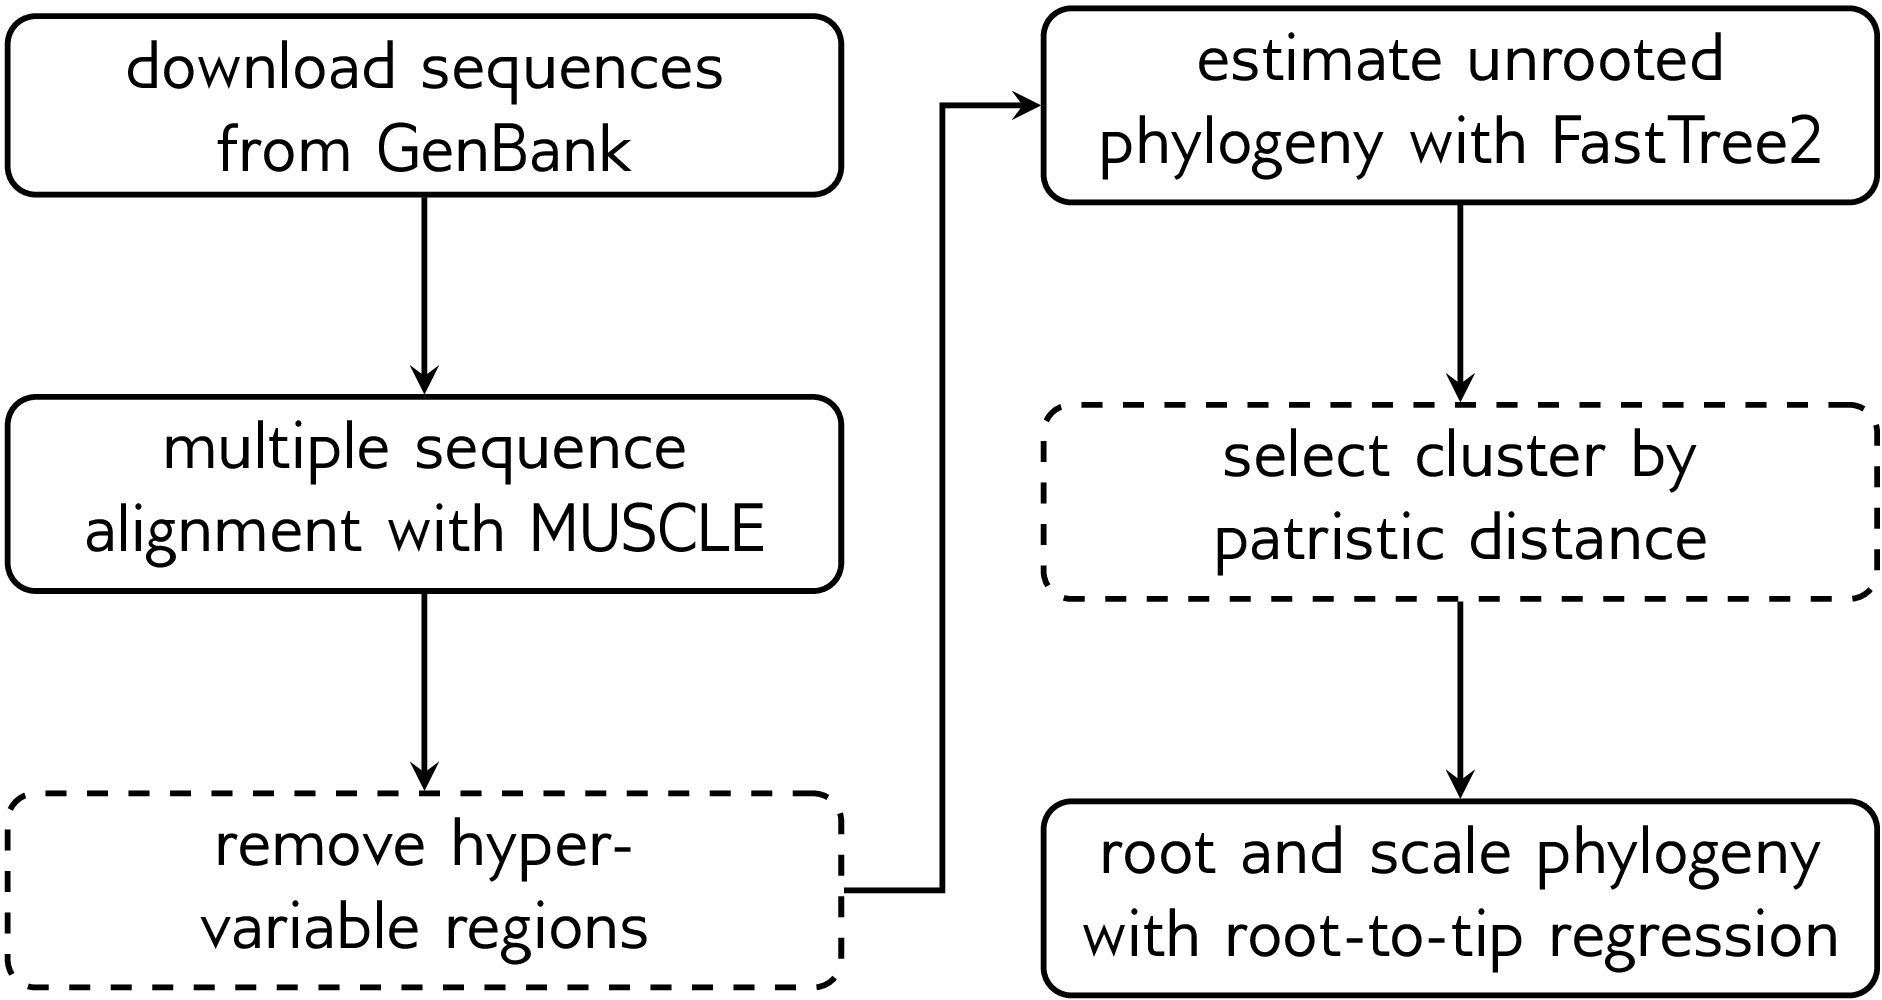
\includegraphics[width=0.2\textwidth]{pipeline}}

    \nocite{edgar2004muscle}
    \nocite{price2010fasttree}
    \nocite{drummond2003inference}
  }

  \block{Parameter heterogeneity among real datasets}{
    \centerline{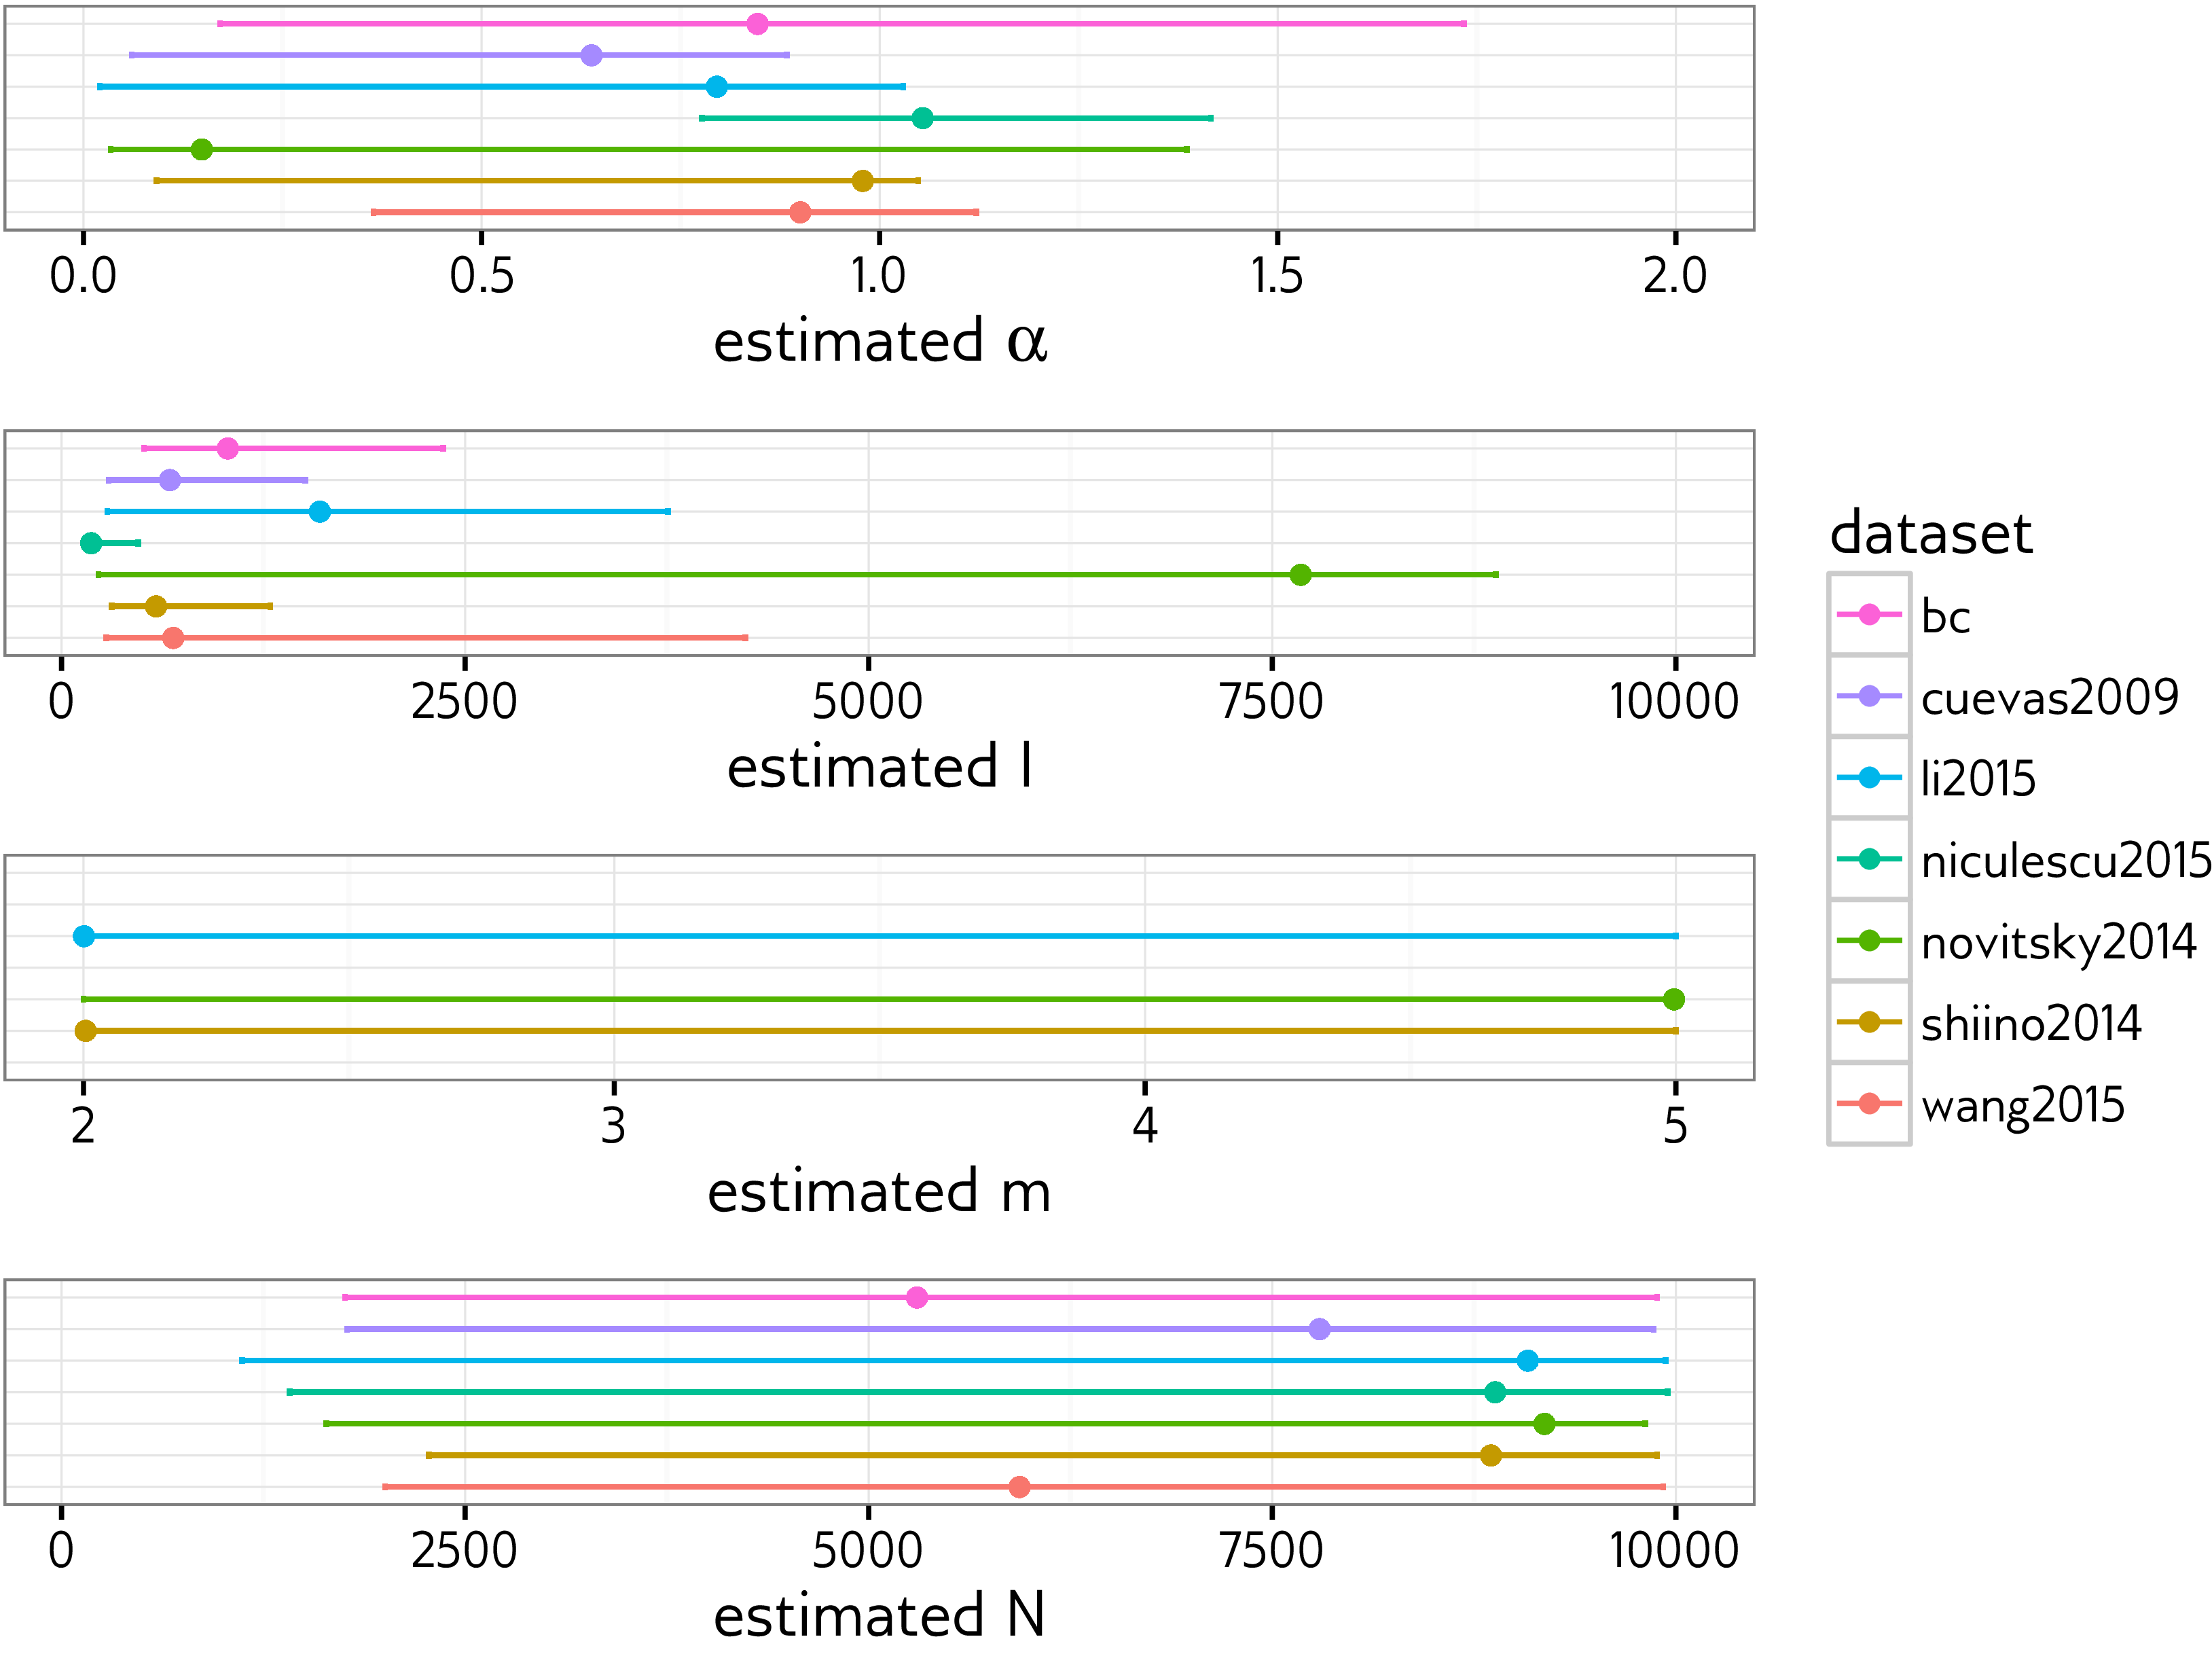
\includegraphics[width=0.2\textwidth]{realdata-hpd-bc}}
  }
\end{columns}

\begin{columns}
  \column{0.6}
  \block{Summary}{
    \Large
    We developed a kernel-ABC method for inference of structural contact
    network parameters from viral sequence data.

    The Barab\'asi-Albert model is one of the simplest preferential attachment
    models which makes a number of unrealistic modelling assumptions. In
    particular, the average degree of the network is equal to $2m$, which is
    constrained to a multiple of 2. Moreover, we assume that the network is
    static and connected, and that nodes are never removed and are homogeneous
    in their behaviour. These assumptions mean that the model is very likely
    misspecified for the real data in question. However, method can be applied
    to any network model from which simulations can be drawn, leaving open the
    possibility to investigate more realistic models in the future.
  }

  \column{0.4}
  \block{References} {
    \printbibliography[heading=none]
  }
  \block{Funding and acknowledgements} {
    some logos
  }
\end{columns}

\end{document}
